\begin{figure*}
\scriptsize{
\medskip
%%%%%%%%%%%%%%%%%%%%
$
\inferrule
{
}
{\Refines;\AvailableActions \vdash \skipstmt \leadsto \skipstmt}
\;(\textsc{Skip})
$
\medskip
%%%%%%%%%%%%%%%%%%%%
$
\inferrule
{
}
{\Refines;\AvailableActions \vdash \assert{\locExpr} \leadsto \assert{\locExpr}}
\;(\textsc{Assert})
$
\medskip
%%%%%%%%%%%%%%%%%%%%
$
\inferrule
{
}
{\Refines;\AvailableActions \vdash \yield{e,\lins} \leadsto \yield{e,\lins}}
\;(\textsc{Yield})
$
\medskip
%%%%%%%%%%%%%%%%%%%%
$
\inferrule
{
A \in \AvailableActions
}
{\Refines;\AvailableActions \vdash \call{A} \leadsto \call{A}}
\;(\textsc{Atomic})
$
\medskip
%%%%%%%%%%%%%%%%%%%%
$
\inferrule
{
\Refines;\AvailableActions \vdash s \leadsto s'
}
{
\Refines;\AvailableActions \vdash \ablock{e,\lins}{s} \leadsto s'
}
\;(\textsc{Ablock-Elim})
$
\medskip
%%%%%%%%%%%%%%%%%%%%
$
\inferrule
{
\Refines;\AvailableActions \vdash s \leadsto s'
}
{
\Refines;\AvailableActions \vdash s \leadsto \ablock{e,\lins}{s'}
}
\;(\textsc{Ablock-Intro})
$
\medskip
%%%%%%%%%%%%%%%%%%%%
$
\inferrule
{
P \in \dom(\Refines)
}
{
\Refines;\AvailableActions \vdash \call{P} \leadsto \call{\Refines(P)}
}
\;(\textsc{Proc1})
$
\medskip
%%%%%%%%%%%%%%%%%%%%
$
\inferrule
{
P \not\in \dom(\Refines)
}
{
\Refines;\AvailableActions \vdash \call{P} \leadsto \call{P}
}
\;(\textsc{Proc2})
$
\medskip
%%%%%%%%%%%%%%%%%%%%
$
\inferrule
{
P \not\in \dom(\Refines)
}
{
\Refines;\AvailableActions \vdash \async{P} \leadsto \async{P}
}
\;(\textsc{Async})
$
\medskip
%%%%%%%%%%%%%%%%%%%%
$
\inferrule
{
\Refines;\AvailableActions \vdash \StmtStack \leadsto \StmtStack'
}
{
\Refines;\AvailableActions \vdash (\varsL,\StmtStack) \leadsto (\varsL,\StmtStack')
}
\;(\textsc{Stack})
$
\medskip
%%%%%%%%%%%%%%%%%%%%
$
\inferrule
{
\Refines;\AvailableActions \vdash \StmtStack \leadsto \StmtStack' \\
\Refines;\AvailableActions \vdash \stmt \leadsto \stmt'
}
{
\Refines;\AvailableActions \vdash \StmtStack;\stmt \leadsto \StmtStack';\stmt'
}
\;(\textsc{Seq})
$
\medskip
%%%%%%%%%%%%%%%%%%%%
$
\inferrule
{
\Refines;\AvailableActions \vdash s_1 \leadsto s_1' \\
\Refines;\AvailableActions \vdash s_2 \leadsto s_2'
}
{
\Refines;\AvailableActions \vdash \ite{\locExpr}{s_1}{s_2} \leadsto \ite{\locExpr}{s_1'}{s_2'}
}
\;(\textsc{Ite})
$
\medskip
%%%%%%%%%%%%%%%%%%%%
$
\inferrule
{
\Refines;\AvailableActions \vdash s \leadsto s'
}
{
\Refines;\AvailableActions \vdash \while{e,\alpha}{\locExpr}{s} \leadsto \while{e,\alpha}{\locExpr}{s'}
}
\;(\textsc{While})
$
\medskip
%%%%%%%%%%%%%%%%%%%%
$
\inferrule
{
\Refines;\AvailableActions \vdash \stmt \leadsto \stmt'
}
{
\Refines;\AvailableActions \vdash (\phi,\mods,\psi,\stmt) \leadsto (\phi',\mods',\psi',\stmt')
}
\;(\textsc{Procedure})
$
\medskip
%%%%%%%%%%%%%%%%%%%%
$
\inferrule
{
\Refines;\AvailableActions \vdash \StmtStack \leadsto \StmtStack'
}
{
\Refines;\AvailableActions \vdash (\varsTL, (\varsL, \StmtStack)) \leadsto (\varsTL, (\varsL, \StmtStack'))
}
\;(\textsc{Thread})
$
\medskip\\
%%%%%%%%%%%%%%%%%%%%
$
\inferrule
{
\range(\Refines) \subseteq \AvailableActions \\
\forall (\rho,\alpha,m) \in \range(\actions \circ \Refines).\ (\accessVars(\rho) \cap \Local = \emptyset) \wedge (\alpha = ((\elim{\Local}.\ \alpha) \wedge \Same(\Local))) \\
\forall A \in \AvailableActions.\ \actions(A) = \actions'(A) \\
\forall 1 \le i \le n.\ \Refines;\AvailableActions \vdash T_i \leadsto T_i' \\
\forall P \not\in \dom(\Refines).\ \Refines;\AvailableActions \vdash \procs(P) \leadsto \procs'(P)
}
{
\Refines;\AvailableActions \vdash (\procs, \actions, \ProcLins, \varsG, T_1 \ldots T_n) \leadsto (\procs', \actions', \ProcLins', \varsG, T_1' \ldots T_n')
}
\;(\textsc{Program})
$
\medskip
%%%%%%%%%%%%%%%%%%%%
}
\caption{Program transformation}
\label{fig:program-transformation}
\end{figure*}

Suppose a program $\Prog'$ has been proved to be safe.
However, it is implemented using atomic actions that are too coarse to be directly implementable.  
To carry over the safety of $\Prog'$ to a realizable implementation $\Prog$, 
these coarse atomic actions must be refined down to lower-level actions.
During this refinement, an invocation $\call{A}$ of a high-level atomic action $A$ is transformed into an 
invocation $\call{P}$ of a procedure that is implemented using low-level actions.
The main contribution of this paper is a verification method that allows us to safely refine
program $\Prog'$ to another program $\Prog$ so that 
safety properties proved on $\Prog'$ continue to hold on $\Prog$ as well.

We formalize the program transformation connecting $\Prog$ to $Prog'$ as a judgment
$\Refines;\AvailableActions \vdash \Prog \leadsto \Prog'$;
the rules for this judgment are presented in Figure~\ref{fig:program-transformation}.
In this judgment,
$\Refines \in \ProcName \pf \ActionName$ is a partial function from procedure names to action names
and $\AvailableActions \in 2^{\ActionName}$ is a set of action names $\range(\Refines)$.
This judgment expresses the intention that $\Prog$ is abstracted by replacing
occurrences of $\call{P}$ with $\call{\Refines(P)}$ for all $P \in \dom(\Refines)$ such that 
the resulting program $\Prog'$ uses only actions in $\AvailableActions$.
Consequently, the procedures in $\dom(\Refines)$ are not used in $\Prog'$.

Rule \textsc{Program} checks that $\range(\Refines) \subseteq \AvailableActions$,
which ensures that $\Prog'$ only uses actions in $\AvailableActions$.
It also checks that every action in $\range(\Refines)$ has a precondition 
that is independent of procedure-local variables and a transition relation that leaves 
procedure-local variables unchanged.  
This check is meaningful because the action $\Refines(P)$ is written from the 
perspective of the caller of $P$.
Since the procedure-local variables of the caller of $P$ are distinct from those of $P$,
these variables are quantified out from the transition relation of $\Refines(P)$ when 
the body of $P$ is being checked (see Section~\ref{sec:refinement}).
The judgment uses the notation $\elim{\Local}.\ \alpha$, defined to be the following transition relation:
\[\{(\MakeStore{\varsG}{\varsTL}{\varsL}, \MakeStore{\varsG'}{\varsTL'}{\varsL'}) \mid \exists \varsL_1,\varsL_2.\ (\MakeStore{\varsG}{\varsTL}{\varsL_1}, \MakeStore{\varsG'}{\varsTL'}{\varsL_2}) \in \alpha \}.\]
Finally, this rule constrains actions in $\AvailableActions$ to be identical and then rewrites all threads
and all procedures that continue to be used in $\Prog'$.

Rule \textsc{Thread}

The program transformation $\Prog \leadsto \Prog'$ is clearly not sound by itself.
To justify the transformation, a collection of auxiliary judgments need to be proved.
We now present an overview of these judgments.
The judgment $\vdash \Prog$, described in Section~\ref{sec:linearity}, 
checks that $\Prog$ uses linear variables appropriately and that the statement
inside any atomic block does not contain any yield.
The former is important because appropriate use of linear variables gives our verifier access to free disjointness
assumptions that are important for precise non-interference and commutativity reasoning (as described later in this section).
The latter is important because non-interference between threads is checked pairwise by verifying that each yield predicate
in one thread is preserved by each atomic block in a different thread.

Next, we have three judgments, $\Refines \jr \Prog$, $\Refines \js \Prog$, and $\InterferenceFree(\Prog, \Refines)$,
described in Section~\ref{sec:refinement},
that together establish that all program annotations are consistent and that 
each occurrence of $\call{P}$ in $\Prog$ behaves like $\call{\Refines(P)}$ 
for all $P \in \dom(\Refines)$.
The rules for these judgments generalize the method of Owicki and Gries~\cite{OwickiG76} for reasoning about concurrent programs.
The judgment $\Refines \js \Prog$ checks sequential correctness of each computation;
the judgment $\InterferenceFree(\Prog, \Refines)$ checks that each thread preserves the
yield predicate of every other thread;
the judgment $\Refines \jr \Prog$ uses the assertions established by the previous two judgments to check that 
the code of procedure $P$ behaves like the atomic action $\Refines(P)$ for all $P\in\dom(\Refines)$.

Finally, we have two judgments $\CommutativitySafe(\Prog)$ and $\Refines \jy \Prog$, 
described in Section~\ref{sec:yield-elimination}, that allow us to further simplify reasoning 
about the abstract program $\Prog'$ by soundly eliminating yields between the invocations of atomic actions in $\range(\Refines)$.
Yield elimination is extremely important to reduce the complexity of annotations and invariants 
required for proving the correctness of concurrent programs;
in our framework, it would be useful for simplifying the proof of the abstract program $\Prog'$.
We use commutativity reasoning on definitions of atomic actions and their declared mover types~\cite{FlanaganFLQ08,ElmasQT09}
to perform yield elimination soundly.

In the remainder of this section, we will formalize the judgments discussed above
and present our soundness theorem in Section~\ref{sec:correctness}.

\subsection{Using linear variables}
\label{sec:linearity}

\begin{figure*}
\scriptsize{
\medskip
%%%%%%%%%%%%%%%%%%%%
$
\inferrule
{
}
{
\lins;\ABlockAny \vdash \skipstmt : \lins
}
\;(\textsc{Skip})
$
\medskip
%%%%%%%%%%%%%%%%%%%%
$
\inferrule
{
}
{
\lins;\ABlockOutside \vdash \assert{\locExpr} : \lins
}
\;(\textsc{Assert})
$
\medskip
%%%%%%%%%%%%%%%%%%%%
$
\inferrule
{
\lins_y \subseteq \lins
}
{
\lins;\ABlockOutside \vdash \yield{e,\lins_y} : \lins
}
\;(\textsc{Yield})
$
\medskip
%%%%%%%%%%%%%%%%%%%%
$
\inferrule
{
\ProcLins(A) = (\lins,\lins')
}
{
\lins;\ABlockInside \vdash \call{A} : \lins'
}
\;(\textsc{Atomic})
$
\medskip
%%%%%%%%%%%%%%%%%%%%
$
\inferrule
{
\ProcLins(P) = (\lins,\lins') \\
}
{
\lins;\ABlockOutside \vdash \call{P} : \lins'
}
\;(\textsc{Proc})
$
\medskip
%%%%%%%%%%%%%%%%%%%%
$
\inferrule
{
\lins_G \subseteq \Global \\
\lins \cup \lins_P \cup \lins_P' \subseteq \ThreadLocal \\
\ProcLins(P) = ((\lins_G,\lins_P),(\lins_G,\lins_P')) \\
}
{
\lins_G,\lins,\lins_P;\ABlockOutside \vdash \async{P} : \lins_G,\lins
}
\;(\textsc{Async})
$
\medskip
%%%%%%%%%%%%%%%%%%%%
$
\inferrule
{
\lins;\ABlockInside \vdash \stmt : \lins' \\
\lins_a \subseteq \lins
}
{
\lins;\ABlockOutside \vdash \ablock{e,\lins_a}{\stmt} : \lins'
}
\;(\textsc{Ablock})
$
\medskip
%%%%%%%%%%%%%%%%%%%%
$
\inferrule
{
\lins;\ABlockAny \vdash \StmtStack : \lins'
}
{
\lins;\ABlockAny \vdash (\varsL,\StmtStack) : \lins'
}
\;(\textsc{Stack})
$
\medskip
%%%%%%%%%%%%%%%%%%%%
$
\inferrule
{
\lins;\ABlockAny \vdash \StmtStack : \lins' \\
\lins';\ABlockAny \vdash \stmt : \lins''
}
{
\lins;\ABlockAny \vdash \StmtStack;\stmt : \lins''
}
\;(\textsc{Seq})
$
\medskip
%%%%%%%%%%%%%%%%%%%%
$
\inferrule
{
\lins;\ABlockAny \vdash \stmt_1 : \lins' \\
\lins;\ABlockAny \vdash \stmt_2 : \lins'
}
{
\lins;\ABlockAny \vdash \ite{\locExpr}{\stmt_1}{\stmt_2} : \lins'
}
\;(\textsc{Ite})
$
\medskip
%%%%%%%%%%%%%%%%%%%%
$
\inferrule
{
\lins;\ABlockAny \vdash \stmt : \lins
}
{
\lins;\ABlockAny \vdash \while{e,\alpha}{\locExpr}{\stmt} : \lins
}
\;(\textsc{While})
$
\medskip
%%%%%%%%%%%%%%%%%%%%
$
\inferrule
{
\ProcLins(P) = (\lins,\lins') \\
\procs(P) = (\phi, \mods, \psi, \stmt) \\
\lins;\ABlockOutside \vdash \stmt : \lins'
}
{
\vdash P
}
\;(\textsc{Procedure})
$
\medskip
%%%%%%%%%%%%%%%%%%%%
$
\inferrule
{
T = (\varsTL, (\varsL, \StmtStack)) \\
\lins;\ABlockOutside \vdash \StmtStack : \lins'
}
{
\lins \vdash T
}
\;(\textsc{Thread})
$
\medskip
%%%%%%%%%%%%%%%%%%%%
$
\inferrule
{
\ProcLins(A) = (\lins,\lins') \\
\lins \cap \Global = \lins' \cap \Global \\
\actions(A) = (\rho, \alpha, m) \\\\
\forall (\sigma,\sigma') \in \alpha.\ 
  \disjoint(\{\sigma(x) \mid x \in \lins\}) \Rightarrow
  \disjoint(\{\sigma'(x) \mid x \in \lins'\}) \\
\forall (\sigma,\sigma') \in \alpha.\ 
  \bigcup\{\sigma'(x) \mid x \in \lins'\} \subseteq \bigcup\{\sigma(x) \mid x \in \lins\}
}
{
\vdash A
}
\;(\textsc{Action})
$
\medskip
%%%%%%%%%%%%%%%%%%%%
$
\inferrule
{
\forall P \in \ProcName. \vdash P \\
\forall A \in \ActionName. \vdash A \\
\lins_G \subseteq \Global \\
\forall 1 \le i \le n. (\lins_i \subseteq \ThreadLocal) \\
\forall 1 \le i \le n. (\lins_G,\lins_i \vdash T_i) \\
\forall 1 \le i \le n. (T_i = (\varsTL_i, \ldots)) \\
\disjoint(\{\varsG(x) \mid x \in \lins_G\} \cup
  \{\varsTL_i(x) \mid 1 \le i \le n, x \in \lins_i\})
}
{
\vdash (\procs, \actions, \ProcLins, \varsG, T_1 \ldots T_n)
}
\;(\textsc{Program})
$
\medskip
%%%%%%%%%%%%%%%%%%%%
}
\caption{Linear variables and atomic blocks}
\label{fig:linearity}
\end{figure*}

In this section, we formalize the judgment $\vdash \Prog$.
The rules for this judgment, presented in Figure~\ref{fig:linearity}, check that
linear variables and atomic blocks are used appropriately in $\Prog$.
Starting from the bottom of Figure~\ref{fig:linearity}, rule \textsc{Program} checks 
all procedures, actions, and threads in $\Prog$.
To check a thread $T_i$, the initial set of linear permissions, global and thread-local,
are required. 
The rule guesses a set of global linear variables $\lins_G$
and a set of thread-local linear variables $\lins_i$ and checks $T_i$ in an environment
containing their union $\lins_G,\lins_i$.
Rule \textsc{Program} uses the predicate $\disjoint(\Lambda)$ where $\Lambda$ is a subset 
of $\Global \cup \ThreadLocal$.
This predicate is used to encode a disjointness invariant enforced by the linear type checker
with respect to an arbitrary function $\Set$ (provided by the programmer) from $\Value$ to $2^\Value$.
$\disjoint(\Lambda)$ states that the sets $\Set(\lins)$ for $\lins \in \Lambda$ are pairwise disjoint.
The judgment $\vdash \Prog$ enforces that linear permissions are never duplicated during the 
execution of $\Prog$.
Rule \textsc{Program} also checks that the disjointness invariant holds in the initial state of $\Prog$.
Consequently, it holds throughout the execution of $\Prog$.

Rule \textsc{Action} checks each action $A$ locally, using its linear interface $(\lins,\lins')$,
to ensure that it does violate the disjointness invariant.
%Since only actions can update the program store, this check suffices to ensure the preservation of the
%invariant throughout the program's execution.
There are three conditions being checked.
First, the set of global linear permissions does not change from the input to the output.
Second, if the disjointness invariant holds for input permissions it also holds for output permissions.
Finally, the union of the sets constructed from output permissions is a subset of the union of sets
constructed from input permissions.  
This last condition is important because it allows via local checking to conclude that the disjointness invariant holds globally
for linear permissions held by all threads.

Rule \textsc{Thread} checks the statement stack $\StmtStack$ inside a thread
with the initial set of linear permissions $\lins$ handed down by rule \textsc{Program} 
and an arbitrary set of final permissions $\lins'$.
In addition to appropriate usage of linear variables, it also checks that each atomic block does not contain any 
occurrences of $\mathit{yield}$, $\mathit{call}$, or $\mathit{async}$ statements inside it.
This latter check is performed by introducing another parameter, one of two values in $\{\ABlockOutside,\ABlockInside\}$, 
to the judgment.
$\ABlockOutside$ states that the current statement is outside any atomic block;
$\ABlockInside$ states that the current statement is inside some atomic block.
Rule \textsc{Procedure} is similar to the rule \textsc{Thread};
it checks the procedure body against its linear interface.
Both these rules use $\ABlockOutside$ to indicate that the current control is outside any atomic block.
Proper usage of atomic blocks requires that 
(1)~any invocation of an atomic action (the only computation that can modify the store) must occur inside an atomic block, and
(2)~any $\mathit{yield}$, $\mathit{call}$, $\mathit{async}$, or $\mathit{assert}$ statements must occur outside all atomic blocks.
These two requirements together provide two simplifications that we exploit in Section~\ref{sec:refinement}.
First, an atomic block cannot fail and can therefore be summarized by a transition relation.
Second, checking non-interference of a yield predicate against all atomic blocks concurrently executing 
in the environment will preserve the yield predicate across the entire computation across a context switch by the environment.

Rules \textsc{Stack}, \textsc{Seq}, \textsc{Ite}, and \textsc{While} are straightforward.
Rule \textsc{Ablock} checks that the linear permissions associated with the atomic block are available
and then checks the body of the atomic block in the context $\ABlockInside$.
Note that we do not allow nested atomic blocks as indicated by the presence of $\ABlockOutside$ below the line.
The rule \textsc{Async} splits the thread-local permissions $\lins$ of the caller of $\async{P}$ into $\lins$ 
and $\lins_P$, passing $\lins_P$ to the new thread and continuing with $\lins$.
Note that all global permissions in $\lins_G$ are also made available to the new thread;
there is no duplication because all threads refer to the same set of global variables.
The checking of permissions in all the other rules \textsc{Skip}, \textsc{Assert}, \textsc{Yield}, \textsc{Atomic}, and \textsc{Proc}
is straightforward.

\subsection{Refinement}
\label{sec:refinement}

\begin{figure}
\scriptsize{
\medskip
%%%%%%%%%%%%%%%%%%%%
$
\inferrule
{
}
{\actions \vdash \skipstmt \preceq \Havoc(\{\})}
\;(\textsc{Skip})
$
\medskip
%%%%%%%%%%%%%%%%%%%%
$
\inferrule
{
}
{\actions \vdash \assert{\locExpr} \preceq \Havoc(\{\})}
\;(\textsc{Assert})
$
\medskip
%%%%%%%%%%%%%%%%%%%%
$
\inferrule
{
}
{\actions \vdash \yield{e,\lins} \preceq \false}
\;(\textsc{Yield})
$
\medskip
%%%%%%%%%%%%%%%%%%%%
$
\inferrule
{
\actions(A) = (\rho, \alpha, m) 
}
{\actions \vdash \call{A} \preceq \alpha}
\;(\textsc{Atomic})
$
\medskip
%%%%%%%%%%%%%%%%%%%%
$
\inferrule
{
}
{\actions \vdash \call{P} \preceq \false}
\;(\textsc{Call})
$
\medskip
%%%%%%%%%%%%%%%%%%%%
$
\inferrule
{
}
{\actions \vdash \async{P} \preceq \Havoc(\{\})}
\;(\textsc{Async})
$
\medskip
%%%%%%%%%%%%%%%%%%%%
$
\inferrule
{
s \preceq \alpha
}
{\actions \vdash \ablock{e,\lins}{s} \preceq \alpha}
\;(\textsc{Ablock})
$
\medskip
%%%%%%%%%%%%%%%%%%%%
$
\inferrule
{
\actions \vdash \stmt_1 \preceq \alpha_1 \\\\ \actions \vdash \stmt_2 \preceq \alpha_2
}
{\actions \vdash \stmt_1;\stmt_2 \preceq \alpha_1 \circ \alpha_2}
\;(\textsc{Seq})
$
\medskip
%%%%%%%%%%%%%%%%%%%%
$
\inferrule
{
\actions \vdash \stmt_1 \preceq \ga{\locExpr}{\alpha_1} \\ \actions \vdash \stmt_2 \preceq \ga{\neg \locExpr}{\alpha_2}
}
{\actions \vdash \ite{\locExpr}{\stmt_1}{\stmt_2} \preceq \alpha_1 \vee \alpha_2}
\;(\textsc{Ite})
$
\medskip
%%%%%%%%%%%%%%%%%%%%
$
\inferrule
{
\actions \vdash \stmt \preceq \beta \\ \neg \locExpr \circ \Havoc(\{\}) \Rightarrow \alpha \\ \beta \circ \alpha \Rightarrow \alpha 
}
{\actions \vdash \while{e,\alpha}{\locExpr}{\stmt} \preceq e \circ \alpha \circ \neg \locExpr}
\;(\textsc{While})
$
\medskip
%%%%%%%%%%%%%%%%%%%%
$
\inferrule
{
\actions \vdash \stmt \preceq \alpha \\ \alpha \Rightarrow \alpha'
}
{\actions \vdash \stmt \preceq \alpha'}
\;(\textsc{Weaken})
$
\medskip
}
\caption{Statement summarization}
\label{fig:statement-summarization}
\end{figure}

\begin{figure}
\scriptsize{
\medskip
%%%%%%%%%%%%%%%%%%%%
$
\inferrule
{
}
{\Refines;\actions;P \jr \skipstmt : \false}
\;(\textsc{Skip})
$
\medskip
%%%%%%%%%%%%%%%%%%%%
$
\inferrule
{
}
{\Refines;\actions;P \jr \assert{\locExpr} : \false}
\;(\textsc{Assert})
$
\medskip
%%%%%%%%%%%%%%%%%%%%
$
\inferrule
{
}
{\Refines;\actions;P \jr \yield{e,\lins} : \false}
\;(\textsc{Yield})
$
\medskip
%%%%%%%%%%%%%%%%%%%%
$
\inferrule
{
P' \in \dom(\Refines) \\ \actions(\Refines(P')) = (\rho',\alpha',m) \\\\ \rho' \circ \alpha' \Rightarrow \Havoc(\Local)
}
{\Refines;\actions;P \jr \call{P'} : \false}
\;(\textsc{Call1})
$
\medskip
%%%%%%%%%%%%%%%%%%%%
$
\inferrule
{
P' \in \dom(\Refines) \\ \actions(\Refines(P)) = (\rho,\alpha,m) \\ 
\actions(\Refines(P')) = (\rho',\alpha',m) \\ \rho' \circ \alpha' \Rightarrow \elim{\Local}.\ \alpha
}
{\Refines;\actions;P \jr \call{P'} : \true}
\;(\textsc{Call2})
$
\medskip
%%%%%%%%%%%%%%%%%%%%
$
\inferrule
{
P' \in \dom(\Refines) \\ \actions(\Refines(P')) = (\rho',\alpha',m) \\ \rho' \circ \alpha' \Rightarrow \Havoc(\Local)
}
{\Refines;\actions;P \jr \async{P'} : \false}
\;(\textsc{Async})
$
\medskip
%%%%%%%%%%%%%%%%%%%%
$
\inferrule
{
\actions \vdash s \preceq \ga{e}{\Havoc(\Local)}
}
{\Refines;\actions;P \jr \ablock{e,\lins}{s} : \false}
\;(\textsc{Ablock1})
$
\medskip
%%%%%%%%%%%%%%%%%%%%
$
\inferrule
{
\actions(\Refines(P)) = (\rho,\alpha,m) \\\\
\actions \vdash s \preceq \ga{e}{\elim{\Local}.\ \alpha}
}
{\Refines;\actions;P \jr \ablock{e,\lins}{s} : \true}
\;(\textsc{Ablock2})
$
\medskip
%%%%%%%%%%%%%%%%%%%%
$
\inferrule
{
\Refines;\actions;P \jr \stmt_1 : b_1 \\ \Refines;\actions;P \jr \stmt_2 : b_2 \\ \neg(b_1 \wedge b_2)
}
{\Refines;\actions;P \jr \stmt_1;\stmt_2 : b_1 \vee b_2}
\;(\textsc{Seq})
$
\medskip
%%%%%%%%%%%%%%%%%%%%
$
\inferrule
{
\Refines;\actions;P \jr \stmt_1 : b \\ \Refines;\actions;P \jr \stmt_2 : b
}
{\Refines;\actions;P \jr \ite{\locExpr}{\stmt_1}{\stmt_2} : b}
\;(\textsc{Ite})
$
\medskip
%%%%%%%%%%%%%%%%%%%%
$
\inferrule
{
\Refines;\actions;P \jr \stmt : \false
}
{\Refines;\actions;P \jr \while{e,\alpha}{\locExpr}{\stmt} : \false}
\;(\textsc{While})
$
\medskip
%%%%%%%%%%%%%%%%%%%%
$
\inferrule
{
\procs(P) = (\phi, \mods, \psi, \stmt) \\\\
\forall P \in \dom(\Refines).\ \Refines;\actions;P \jr \stmt : \true
}
{
\Refines \jr (\procs, \actions, \ProcLins, \varsG, T_1 \ldots T_n)
}
\;(\textsc{Program})
$
\medskip
%%%%%%%%%%%%%%%%%%%%
}
\caption{Refinement}
\label{fig:refinement}
\end{figure}

In this section, we formalize the judgments $\Refines \jr \Prog$, $\Refines \js \Prog$, and $\InterferenceFree(\Prog,\Refines)$.
The rules for the judgment $\Refines \jr \Prog$, presented in Figure~\ref{fig:refinement}, check that the body of 
each procedure $P$ in $\dom(\Refines)$ behaves like the atomic action $\Refines(P)$.  
Suppose $P$ is a procedure in $\dom(\Refines)$, $A = \Refines(P)$, and $\actions(A) = (\rho, \alpha, m)$.
Our strategy for $P$ is to check that along all paths in its body, there occurs exactly one atomic block 
$\ablock{e,\lins}{\stmt}$ that is simulated by the transition relation $\alpha$.
All other atomic blocks before or after this unique block are simulated by the transition relation $\Havoc(\Local)$ 
which allows procedure-local variables to be modified arbitrarily but requires that global and thread-local variables are not modified.
The judgment for simulating a code block with a transition relation is $\actions \vdash \stmt \preceq \alpha$; the rules for this judgment 
are presented in Figure~\ref{fig:statement-summarization}.
In general, it may not be possible to prove that the body $\stmt$ of the atomic block is simulated by $\alpha$.
Contextual information such as the predicate $e$ that is expected to hold when the atomic block begins execution or the invariants
of the loop inside the atomic block may also be needed.
Proving such predicates throughout the program is the job of the judgments $\Refines \js \Prog$ and $\InterferenceFree(\Prog, \Refines)$.
The rules for the former are presented in Figure~\ref{fig:sequential-correctness} and the latter is formalized in text towards the end of this 
subsection.

We first examine the rules for the judgment $\actions \vdash \stmt \preceq \alpha$ in Figure~\ref{fig:statement-summarization}.
We ignore the rules \textsc{Assert}, \textsc{Yield}, \textsc{Call}, \textsc{Async}, and \textsc{Ablock} for now since the 
statements corresponding to these do not occur inside atomic blocks; we will use these rules later in Section~\ref{sec:yield-elimination}.
The rule \textsc{Skip} states that $\skipstmt$ is simulated by the transition relation $\Havoc(\{\})$ which leaves all variables unchanged.
The rule \textsc{Seq} states that if $\stmt_1$ and $\stmt_2$ are simulated by $\alpha_1$ and $\alpha_2$ respectively, 
then $\stmt_1;\stmt_2$ is simulated by the relational composition $\alpha_1 \circ \alpha_2$.
The rule \textsc{Ite} uses the notation $\ga{\locExpr}{\alpha}$ which represents the set of all transitions $(\sigma, \sigma')$ 
such that $\sigma \in \locExpr \Rightarrow (\sigma,\sigma') \in \alpha$.
It states that if $\stmt_1$ is simulated by $\ga{\locExpr}{\alpha_1}$ and $\stmt_2$ is simulated by $\ga{\neg \locExpr}{\alpha_2}$,
then $\ite{\locExpr}{\stmt_1}{\stmt_2}$ is simulated by $\alpha_1 \vee \alpha_2$.
The rule \textsc{While} summarizes the body of the while loop by the transition relation $\beta$ and checks that the 
loop summary $\alpha$ provided by the programmer is inductive.
These checks allow the rule to conclude that the loop is summarized by $e \circ \alpha \circ \neg \locExpr$.
Here (and elsewhere in this section), we overload a predicate $e$ over the store as the transition relation $\{(\sigma,\sigma') \mid \sigma \in e\}$.
Note that the computed loop summary assumes the loop invariant $e$ since it is checked using the other judgments discussed later in this section.

Next we examine the rules for the the judgment $\Refines \jr \Prog$ in Figure~\ref{fig:refinement}.
The crux of these rules is the judgment $\Refines;\actions;P \jr \stmt : b$, 
where $P$ is a procedure in $\dom(\Refines)$, $\stmt$ is a statement inside the body of $P$, and $b$ is a 
$\mathit{Boolean}$ value.
Suppose $\Refines(P) = A$ and $\actions(A) = (\rho, \alpha, m)$.
If $b$ is $\true$, this judgment indicates that during any execution of $\stmt$, 
an atomic block that could be simulated by $\elim{\Local}.\ \alpha$ happened exactly once;
this unique atomic modifies global and thread-local variables as constrained by $\alpha$.
If $b$ is $\false$, this judgment indicates that during any execution of $\stmt$, each atomic block
was simulated by $\Havoc(\Local)$, that is, it did not modify any global or thread-local variables.
Informally, we say that $\stmt$ {\em acts\/} if $b$ is $\true$ and {\em stutters\/} if $b$ is $\false$.

Starting from the bottom, rule \textsc{Program} checks that $\Refines;\actions;P \jr \stmt : \true$
for each $P \in \dom(\Refines)$.
The rule \textsc{While} checks that the body of the loop stutters and concludes that the loop itself stutters.
The rule \textsc{Ite} checks that both branches behave in the same way.
The rule \textsc{Seq} for $\stmt_1;\stmt_2$ guesses the behavior of $\stmt_1$ and $\stmt_2$ but constrains
at most one of them to act.
Rules \textsc{Ablock1} and \textsc{Ablock2} for $\ablock{e,\lins}{s}$ have been described informally in the last paragraph.  
The main difference in the formal rules is that the simulation check is weakened using the predicate $e$
assumed to hold upon entry into the atomic block.
The other interesting rules are \textsc{Call1}, \textsc{Call2}, and \textsc{Async}.
These rules require that the called procedure $P'$ is in $\dom(\Refines)$;
thus, the set of procedures being introduced during refinement must be closed under the call relation.
The rule for ordinary call $\call{P'}$ is similar to that of atomic blocks with the action $\Refines(P')$
taking on the role of the atomic block;
the gate and transition relation of $\Refines(P')$ are used analogously to the predicate and the code of the atomic block.
The rule for asynchronous call $\async{P'}$ checks that $\Refines(P')$ stutters.

{\bf TBD.} discuss $\Refines \js \Prog$ and $\InterferenceFree(\Prog,\Refines)$.

\begin{figure}
\scriptsize{
\medskip
%%%%%%%%%%%%%%%%%%%%
$
\inferrule
{
}
{\procs;\actions;\RefinementAny;\{\} \js \FH{\phi}{\skipstmt}{\phi}}
\;(\textsc{Skip})
$
\medskip\\
%%%%%%%%%%%%%%%%%%%%
$
\inferrule
{
}
{\procs;\actions;\RefinementOutside;\{\} \js \FH{\phi}{\assert{\locExpr}}{\phi}}
\;(\textsc{Assert1})
$
\medskip
%%%%%%%%%%%%%%%%%%%%
$
\inferrule
{
}
{\procs;\actions;\RefinementInside;\{\} \js \FH{\phi \wedge \locExpr}{\assert{\locExpr}}{\phi}}
\;(\textsc{Assert2})
$
\medskip
%%%%%%%%%%%%%%%%%%%%
$
\inferrule
{
}
{\procs;\actions;\RefinementAny;\{\} \js \FH{e}{\yield{e,\lins}}{e}}
\;(\textsc{Yield})
$
\medskip
%%%%%%%%%%%%%%%%%%%%
$
\inferrule
{
\actions(A) = (\rho, \alpha, m) \\ 
\mods \subseteq \ThreadLocal \\
\alpha \Rightarrow \Havoc(\Global \cup \mods \cup \Local) \\
\phi \Rightarrow \rho \\ 
\Unsat{\phi \circ \alpha \circ \neg \psi} \\
}
{\procs;\actions;\RefinementAny;\mods \js \FH{\phi}{\call{A}}{\psi}}
\;(\textsc{Atomic})
$
\medskip
%%%%%%%%%%%%%%%%%%%%
$
\inferrule
{
\procs(P) = (\phi, \mods, \psi, \stmt) \\ P \not \in \dom(\Refines)
}
{\procs;\actions;\RefinementAny;\mods \js \FH{\phi}{\call{P}}{\psi}}
\;(\textsc{Proc1})
$
\medskip
%%%%%%%%%%%%%%%%%%%%
$
\inferrule
{
\procs(P) = (\phi, \mods, \psi, \stmt) \\ P \in \dom(\Refines) \\\\ \procs;\actions;\RefinementAny;\mods \js \FH{\phi}{\call{\Refines(P)}}{\psi}
}
{\procs;\actions;\RefinementAny;\mods \js \FH{\phi}{\call{P}}{\psi}}
\;(\textsc{Proc2})
$
\medskip
%%%%%%%%%%%%%%%%%%%%
$
\inferrule
{
\procs(P) = (\phi, \mods, \psi, \stmt)
}
{\procs;\actions;\RefinementAny;\{\} \js \FH{\rho \wedge \phi}{\async{P}}{\rho}}
\;(\textsc{Async})
$
\medskip\\
%%%%%%%%%%%%%%%%%%%%
$
\inferrule
{
\procs;\actions;\RefinementAny;\mods \js \FH{\phi_1 \wedge e}{s}{\phi_2}
}
{\procs;\actions;\RefinementAny;\mods \js \FH{\phi_1 \wedge e}{\ablock{e,\lins}{s}}{\phi_2}}
\;(\textsc{Ablock})
$
\medskip
%%%%%%%%%%%%%%%%%%%%
$
\inferrule
{
\procs;\actions;\RefinementAny;\mods_1 \js \FH{\phi_1}{\StmtStack}{\phi_2} \\ 
\procs;\actions;\RefinementAny;\mods_2 \js \FH{\phi_2}{s}{\phi_3}
}
{\procs;\actions;\RefinementAny;\mods_1 \cup \mods_2 \js \FH{\phi_1}{\StmtStack;s}{\phi_3}}
\;(\textsc{Seq})
$
\medskip
%%%%%%%%%%%%%%%%%%%%
$
\inferrule
{
\procs;\actions;\RefinementAny;\mods_1 \js \FH{e \wedge \phi_1}{s_1}{\phi_2} \\ 
\procs;\actions;\RefinementAny;\mods_2 \js \FH{\neg e \wedge \phi_1}{s_2}{\phi_2}
}
{\procs;\actions;\RefinementAny;\mods_1 \cup \mods_2 \js \FH{\phi_1}{\ite{\locExpr}{s_1}{s_2}}{\phi_2}}
\;(\textsc{Ite})
$
\medskip
%%%%%%%%%%%%%%%%%%%%
$
\inferrule
{
\procs;\actions;\RefinementAny;\mods \js \FH{e \wedge \locExpr}{s}{e}
}
{\procs;\actions;\RefinementAny;\mods \js \FH{e}{\while{e,\alpha}{\locExpr}{s}}{e \wedge \neg \locExpr}}
\;(\textsc{While})
$
\medskip
%%%%%%%%%%%%%%%%%%%%
$
\inferrule
{
\phi \Rightarrow \phi' \\ \procs;\actions;\RefinementAny;\mods \js \FH{\phi'}{\StmtStack}{\psi'} \\ \psi' \Rightarrow \psi
}
{\procs;\actions;\RefinementAny;\mods \js \FH{\phi}{\StmtStack}{\psi}}
\;(\textsc{Weaken})
$
\medskip
%%%%%%%%%%%%%%%%%%%%
$
\inferrule
{
\procs;\actions;\RefinementAny;\mods \js \FH{\phi}{\StmtStack}{\psi} \\ \accessVars(\rho) \cap \mods = \{\}
}
{\procs;\actions;\RefinementAny;\mods \js \FH{\rho \wedge \phi}{\StmtStack}{\rho \wedge \psi}}
\;(\textsc{Frame})
$
\medskip
%%%%%%%%%%%%%%%%%%%%
$
\inferrule
{
\procs(P) = (\phi, \mods, \psi, \stmt) \\
\RefinementAny = \RefinementInside \Longleftrightarrow P \in \dom(\Refines) \\\\
\procs;\actions;\RefinementAny;\mods' \js \FH{\phi}{\stmt}{\psi} \\
\mods' \subseteq \mods
}
{
\procs;\actions;\Refines \js P
}
\;(\textsc{Procedure})
$
\medskip
%%%%%%%%%%%%%%%%%%%%
$
\inferrule
{
\procs;\actions;\RefinementAny;\mods \js \FH{\phi'}{\StmtStack}{\psi} \\\\
(\accessVars(\phi) \cup \accessVars(\psi)) \cap \Local = \{\} \\\\
\forall \varsG,\varsTL,\varsL.\ \MakeStore{\varsG}{\varsTL}{\varsL} \in \phi \Rightarrow \MakeStore{\varsG}{\varsTL}{\varsL} \in \phi'
}
{
\procs;\actions;\RefinementAny;\mods \js \FH{\phi}{(\varsL',\StmtStack)}{\psi}
}
\;(\textsc{Stack})
$
\medskip
%%%%%%%%%%%%%%%%%%%%
$
\inferrule
{
T = (\varsTL, (\varsL, \StmtStack)) \\
\MakeStore{\varsG}{\varsTL}{\varsL} \in \phi \\
\procs;\actions;\RefinementOutside;\mods \js \FH{\phi}{\StmtStack}{\true}
}
{
\procs;\actions;\varsG \js T
}
\;(\textsc{Thread})
$
\medskip
%%%%%%%%%%%%%%%%%%%%
$
\inferrule
{
\forall P \in \ProcName.\ \procs;\actions;\Refines \js P \\\\
\forall 1 \le i \le n.\ \procs;\actions;\varsG \js T_i
}
{
\Refines \js (\procs, \actions, \ProcLins, \varsG, T_1 \ldots T_n)
}
\;(\textsc{Program})
$
\medskip
%%%%%%%%%%%%%%%%%%%%
}
\caption{Sequential correctness}
\label{fig:sequential-correctness}
\end{figure}

{\bf Non-interference.}
Let $\Prog = (\procs, \actions, \ProcLins, \varsG, \TS)$ be a program
and $\Refines$ be a refinement map.
Let $\Yields(\Prog)$ be the union of the following sets:
\begin{itemize}
\item
$\{(\phi,\lins) \mid \yield{\phi,\lins}~\mathrm{appears~in~\Prog}\}$.
\item
$\{(\phi,\lins) \mid P \in \ProcName \wedge \procs(P) = (\phi, \mods, \psi, \stmt) \wedge \ProcLins(P) = (\lins,\lins')\}$.
\item
$\{(\psi,\lins') \mid P \in \ProcName \wedge \procs(P) = (\phi, \mods, \psi, \stmt) \wedge \ProcLins(P) = (\lins,\lins')\}$.
\end{itemize}
Let $\Ablocks(\Prog,\Refines)$ be the set of atomic blocks in $\Prog$ except those inside the bodies of procedures
in $\dom(\Refines)$.

Let $\FV \subseteq \VarName \setminus \Var$ be a set of fresh variables and $\Subst$ be a one-one 
substitution function from $\ThreadLocal \cup \Local$ to $\FV$.
Let $\Subst(\phi)$ represent the result of applying $\Subst$ to the expression $\phi$.
The program $\Prog$ is interference-free with respect to $\Refines$, denoted by $\InterferenceFree(\Prog,\Refines)$,
if for each predicate ($\phi,\lins_y) \in \Yields(\Prog)$, the following conditions are satisfied:
\begin{enumerate}
\item
For each atomic block $\ablock{e,\lins_a}{s} \in \Ablocks(\Prog,\Refines)$, the judgment
\[
\FH{\Subst(\phi) \wedge e \wedge \disjoint(\Subst(\lins_y \setminus \Global) \cup \lins_a)}{s}{\Subst(\phi)}
\]
holds.
\item
For each $A \in \range(\Refines)$ such that $\actions(A) = (\rho, \alpha, m)$ and $\ProcLins(A) = (\lins_a,\lins'_a)$, 
\[
(\Subst(\phi) \wedge \rho \wedge \disjoint(\Subst(\lins_y \setminus \Global) \cup \lins_a)) \circ \alpha \circ \neg\Subst(\phi)
\]
is unsatisfiable.
\end{enumerate}

\subsection{Yield elimination}
\label{sec:yield-elimination}

\begin{figure}
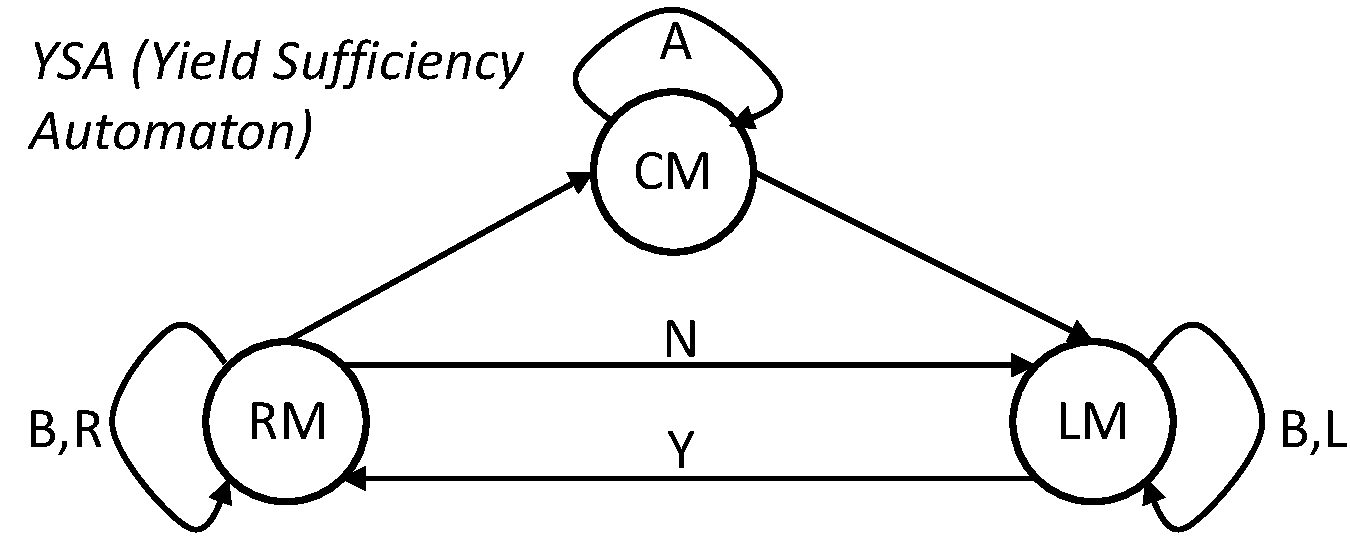
\includegraphics[scale=0.35]{YieldTypeCheckingAutomaton.pdf}
\caption{Automaton for yield sufficiency}
\label{fig:YieldTypeCheckingAutomaton}
\end{figure}

\begin{figure*}
\scriptsize{
\medskip
%%%%%%%%%%%%%%%%%%%%
$
\inferrule
{
}
{\Refines;\actions \jy \skipstmt : (x, x)}
\;(\textsc{Skip})
$
\medskip
%%%%%%%%%%%%%%%%%%%%
$
\inferrule
{
}
{\Refines;\actions \jy \assert{\locExpr} : (x, x)}
\;(\textsc{Assert})
$
\medskip
%%%%%%%%%%%%%%%%%%%%
$
\inferrule
{
}
{\Refines;\actions \jy \yield{e,\lins} : (x, \RM)}
\;(\textsc{Yield})
$
\medskip
%%%%%%%%%%%%%%%%%%%%
$
\inferrule
{
P \not \in \dom(\Refines)
}
{\Refines;\actions \jy \call{P} : (x, \RM)}
\;(\textsc{Call})
$
\medskip
%%%%%%%%%%%%%%%%%%%%
$
\inferrule
{
P \in \dom(\Refines) \\ \actions(\Refines(P)) = (\rho, \alpha, B)
}
{\Refines;\actions \jy \call{P} : (x, x)}
\;(\textsc{Both})
$
\medskip
%%%%%%%%%%%%%%%%%%%%
$
\inferrule
{
P \in \dom(\Refines) \\ \actions(\Refines(P)) = (\rho, \alpha, R)
}
{\Refines;\actions \jy \call{P} : (\RM, \RM)}
\;(\textsc{Right})
$
\medskip
%%%%%%%%%%%%%%%%%%%%
$
\inferrule
{
P \in \dom(\Refines) \\ \actions(\Refines(P)) = (\rho, \alpha, L)
}
{\Refines;\actions \jy \call{P} : (x, \LM)}
\;(\textsc{Left})
$
\medskip
%%%%%%%%%%%%%%%%%%%%
$
\inferrule
{
P \in \dom(\Refines) \\ \actions(\Refines(P)) = (\rho, \alpha, N)
}
{\Refines;\actions \jy \call{P} : (\RM, \LM)}
\;(\textsc{Non})
$
\medskip
%%%%%%%%%%%%%%%%%%%%
$
\inferrule
{
}
{\Refines;\actions \jy \async{P} : (x, \LM)}
\;(\textsc{Async})
$
\medskip
%%%%%%%%%%%%%%%%%%%%
$
\inferrule
{
x \in \{\RM,\CM\}
}
{\Refines;\actions \jy \ablock{e,\lins}{s} : (x, \CM)}
\;(\textsc{Ablock})
$
\medskip
%%%%%%%%%%%%%%%%%%%%
$
\inferrule
{
\Refines;\actions \jy \StmtStack : (x, y) \\ \Refines;\actions \jy s : (y, z)
}
{\Refines;\actions \jy \StmtStack;s : (x, z)}
\;(\textsc{Seq})
$
\medskip
%%%%%%%%%%%%%%%%%%%%
$
\inferrule
{
\Refines;\actions \jy s_1 : (x, y) \\ \Refines;\actions \jy s_2 : (x, y)
}
{\Refines;\actions \jy \ite{\locExpr}{s_1}{s_2} : (x, y)}
\;(\textsc{Ite})
$
\medskip
%%%%%%%%%%%%%%%%%%%%
$
\inferrule
{
\Refines;\actions \jy s : (x, x)
}
{\Refines;\actions \jy \while{e,\alpha}{\locExpr}{s} : (x, x)}
\;(\textsc{While})
$
\medskip
%%%%%%%%%%%%%%%%%%%%
$
\inferrule
{
\procs(P) = (\phi, \mods, \psi, \stmt) \\
\Refines;\actions \jy \stmt : (x, y)
}
{
\Refines;\actions \jy P
}
\;(\textsc{Procedure})
$
\medskip
%%%%%%%%%%%%%%%%%%%%
$
\inferrule
{
\Refines;\actions \jy \StmtStack : (x,y)
}
{
\Refines;\actions \jy (\varsL,\StmtStack) : (x,y)
}
\;(\textsc{Stack})
$
\medskip
%%%%%%%%%%%%%%%%%%%%
$
\inferrule
{
T = (\varsTL, (\varsL, \StmtStack)) \\
\Refines;\actions \jy (\varsL, \StmtStack) : (x, y)
}
{
\Refines;\actions \jy T
}
\;(\textsc{Thread})
$
\medskip
%%%%%%%%%%%%%%%%%%%%
$
\inferrule
{
\forall P \in \ProcName \setminus \dom(\Refines).\ \Refines;\actions \jy P \\\\
\forall 1 \le i \le n.\ \Refines;\actions \jy T_i
}
{
\Refines \jy (\procs, \actions, \ProcLins, \varsG, T_1 \ldots T_n)
}
\;(\textsc{Program})
$
\medskip
%%%%%%%%%%%%%%%%%%%%
}
\caption{Yield elimination}
\label{fig:yield-elimination}
\end{figure*}

Section~\ref{sec:refinement} showed how we can replace a call to a procedure with 
a call to an atomic action.
If each such call to an atomic action had a yield just before and a yield just after it,
we would have a sound transformation of the original program and all safety properties proved
on the abstract program would carry over to the refined program.
However, we can do better by arguing that some of yields surrounding the calls to atomic actions 
are unnecessary by exploiting commutativity properties of the atomic actions.
In this section, we lay out this argument formally.

Let $\Prog = (\procs, \actions, \ProcLins, \varsG, \TS)$ be a program.
The map $\actions$ maps each atomic action to a triple $(\rho, \alpha, m)$, the last component of which 
denotes type of atomic action---$B$ for {\em both mover}, $R$ for {\em right mover}, $L$ for {\em left mover},
and $N$ for {\em non mover}.
Informally, an action labeled $N$ does not commute with other concurrent actions,
an action labeled $L$ commutes to the left (or earlier in time) of other concurrent actions,
an action labeled $R$ commutes to the right (or later in time) of other concurrent actions,
and an action labeled $B$ commutes both to the left and the right of other concurrent actions.
The ability to commute past actions in the environment provides the capability to eliminate yields.
For example, a yield after a right mover or a yield before a left mover is unncessary.

We now formally define the meaning of the commutativity annotations on $\Prog$ described in the previous paragraph.
Let $\FV_1,\FV_2 \subseteq \VarName \setminus \Var$ be two sets of disjoint fresh variables.
Let $\Subst_1$ and $\Subst_2$ be one-one 
substitution functions from $\ThreadLocal \cup \Local$ to $\FV_1$ and $\FV_2$ respectively.
Th program $\Prog$ is commutativity-safe, denoted by $\CommutativitySafe(\Prog)$,
if for all $A_1,A_2 \in \ActionName$ such that $\actions(A_1) = (\rho_1,\alpha_1,m_1)$, $\actions(A_2) = (\rho_2,\alpha_2,m_2)$,
$\ProcLins(A_1) = (\lins_1,\lins'_1)$, and $\ProcLins(A_2) = (\lins_2,\lins'_2)$, 
all of the following conditions are satisfied:
\begin{enumerate}
\item
If $m_1 \in \{B,R\}$ or $m_2 \in \{B,L\}$, then 
\[
\begin{array}{l}
(\Subst_1(\rho_1) \wedge \Subst_2(\rho_2) \wedge \disjoint(\Subst_1(\lins_1 \setminus \Global) \cup \Subst_2(\lins_2)))\ \circ \\
(\Subst_1(\alpha_1) \wedge \Same(\FV_2)) \circ (\Subst_2(\alpha_2) \wedge \Same(\FV_1)) \\ 
\Rightarrow \\
(\Subst_2(\alpha_2) \wedge \Same(\FV_1)) \circ (\Subst_1(\alpha_1) \wedge \Same(\FV_2))
\end{array}
\]
is valid.
\item
If $m_1 \in \{B,R\}$, then 
\[
\begin{array}{l}
\Subst_1(\rho_1) \wedge \disjoint(\Subst_1(\lins_1 \setminus \Global) \cup \Subst_2(\lins_2))\ \circ \\
\Subst_2(\rho_2) \circ (\Subst_2(\alpha_2) \wedge \Same(\FV_1))\ \circ \\
\neg \Subst_1(\rho_1)
\end{array}
\]
is unsatisfiable.
\item
If $m_1 \in \{B,L\}$, then 
\[
\begin{array}{l}
\neg \Subst_1(\rho_1)\ \circ \\
\Subst_2(\rho_2) \circ (\Subst_2(\alpha_2) \wedge \Same(\FV_1))\ \circ \\
\Subst_1(\rho_1) \wedge \disjoint(\Subst_1(\lins'_1 \setminus \Global) \cup \Subst_2(\lins'_2))
\end{array}
\]
is unsatisfiable.
\item
If $m_1 \in \{B, L\}$, then
\[
\forall \sigma \in \rho_1.\ \exists \sigma'.\ (\sigma, \sigma') \in \alpha_1
\]
is valid.
\end{enumerate}

In transforming a refined program $\Prog$ to an abstract program $\Prog'$, a number of atomic actions 
are introduced simultaneously.
Consequently, we may need to eliminate a collection of yields at the same time.
To achieve this goal, we introduce the automaton in Figure~\ref{fig:YieldTypeCheckingAutomaton} that encodes 
all sequences of atomic actions, atomic blocks, and yields with enough yields to capture all behaviors.
The automaton has three states---$\RM$, $\CM$, and $\LM$.
The edge labels belong to the set $\{B,R,L,N,A,Y\}$, where $B$, $R$, $L$, and $N$ represent the various kinds 
of atomic actions described earlier, $A$ represents an atomic block, and $Y$ represents a yield.
The judgment $\Refines;\actions \jy \Prog$ checks that the code in $\Prog$ can be simulated by traces of this automaton.
This automaton allows traces in which {\em transactions\/} are separated by yields;
Each transaction starts with a sequence of right movers (or both movers) and ends with a sequence of left movers (or both movers).
In the middle, it can have either at most one non mover or a sequence of atomic blocks.

The rules for the judgment $\Refines;\actions \jy \Prog$ are presented in Figure~\ref{fig:yield-elimination}.
The essence of these rules is to capture the effect of a computation as a pair $(x,y)$ where $x,y \in \{\RM,\CM,\LM\}$;
the meaning is that to simulate the computation the automaton moves from state $x$ to state $y$.
Rule \textsc{Program} performs checking for all threads and for all procedures not in $\dom(\Refines)$ since these are the 
only procedures that remain in the abstract program.
Rules \textsc{Thread}, \textsc{Stack}, and \textsc{Procedure} are straightforward.
Rule \textsc{While} checks that the body of the loop leaves the state of the automaton unchanged.
Rule \textsc{Ite} checks that the effect both branches is the same.
Rule \textsc{Seq} composes the effect of $\stmt_1$ with the effect of $\stmt_2$.
Rules \textsc{Both}, \textsc{Right}, \textsc{Left}, \textsc{Non}, and \textsc{Ablock} essentially 
examine the available edges in the automaton to validate the statement and calculate its effect.
Rule \textsc{Async} is interesting because it treats an asynchronous call as a left mover.
Rules \textsc{Yield} and \textsc{Call} treat their statements as a yield.
Rules \textsc{Skip} and \textsc{Assert} leave the state of the automaton unchanged.

The judgment $\Refines;\actions \jy \Prog$ is not quite enough to eliminate yields soundly.
Consider the following program with a global variable {\tt x}, a thread-local variable {\tt t},
a procedure {\tt Nop}, and two threads (shown on the left).
\begin{tabular}{lll}
\begin{tabular}[t]{l}
{\tt [ x := 0 ];} \\
{\tt yield;} \\
{\tt [ t := x ];} \\
{\tt assert t == 0;} \\
{\tt yield;} \\
\end{tabular} 
&
\begin{tabular}[t]{l}
{\tt yield;} \\
{\tt [x := x + 1];} \\
{\tt while (true) } \\
{\tt ~~call Nop;} \\
{\tt yield;} \\
\end{tabular} 
&
\begin{tabular}[t]{l}
{\tt procedure Nop()} \\
{\tt ~~refines [~]} \\
{\tt ~~\{~\}}
\end{tabular}
\end{tabular}
The first thread sets {\tt x} to $0$ in an atomic action (indicated {\tt [x := 0]}),
yields, reads {\tt x} into {\tt t}, and asserts that {\tt t == 0}.
At the yield, the second thread may be scheduled; it changes {\tt x} to $1$ and then calls
{\tt Nop} repeatedly in an infinite loop.
Our method allows {\tt Nop} to be abstracted by the atomic action {\tt [~]} which does nothing
and is clearly a left mover (in fact, a both mover).
As a result, the code of the program will satisfy the yield elimination check described earlier.
However, the program as shown fails because of the implicit yields at the boundaries of {\tt Nop},
whereas replacing {\tt call Nop} with the action {\tt [~]} does not fail.

To address this soundness problem in the presence of left and both movers, we require additionally 
that the abstract program is responsive (formally defined at the end of Section~\ref{sec:language}),
that is, it yields infinitely often in any infinite execution.
The abstract program in the example above is not responsive.

{\bf TBD.} We revise the \textsc{While} rule in the judgment 
$\procs;\actions;\RefinementAny;\mods \js \Prog$.
\[
\inferrule
{
\procs;\actions;\RefinementAny;\mods \js \FH{e \wedge \locExpr}{s}{e} \\ e \wedge \locExpr \Rightarrow f \geq 0 \\ 
\alpha = \{(\sigma,\sigma') \mid \sigma(f) > \sigma'(f)\} \\ s \preceq \ga{(e \wedge \locExpr)}{\alpha}
}
{\procs;\actions;\RefinementAny;\mods \js \FH{e}{\while{e,\alpha,f}{\locExpr}{s}}{e \wedge \neg \locExpr}}
\;(\textsc{While})
\]

\subsection{Correctness}
\label{sec:correctness}

\begin{theorem}
Let $\Prog$ and $\Prog'$ be two programs, $\Refines \in \ProcName \pf \ActionName$ be a partial function,
and $\AvailableActions \in 2^{\ActionName}$ be a set such that the following conditions are satisfied:
\begin{enumerate}
\item
$\vdash \Prog$ and $\vdash \Prog'$ and $\Refines;\AvailableActions \vdash \Prog \leadsto \Prog'$.
\item
$\Refines \jr \Prog$ and $\Refines \js \Prog$ and $\InterferenceFree(\Prog,\Refines)$.
\item
$\CommutativitySafe(\Prog)$ and $\Refines \jy \Prog$.
\end{enumerate}
If $\Safe(\Prog')$ and $\Responsive(\Prog')$, then $\Safe(\Prog)$.
\end{theorem}

Our soundness theorem, stated above, concludes the safety of $\Prog$ from the safety and responsiveness of $\Prog'$.


